\section{Results}
	\subsection{Simulation testing}
		\subsubsection{Estimation performance with perfect information}
	
	Given perfect information about trends in relative abundance and age composition information, and a deterministic stock-recruitment relationship, \iscam\ was able to estimate 216 parameters without any substantial errors.	  Estimation performance is easily demonstrated by comparing estimates of spawning biomass and fishing mortality rates to the true values that were used to simulate the data.  As shown in Figure \ref{FigSimPlot} estimates of spawning biomass and fishing mortality rates were exactly the same as the true values. There is no measurable difference between the observed and predicted trends in the relative abundance information (Figs. \ref{FigSimPlot}cd).
	
\begin{figure}[!tbp]
	% Requires \usepackage{graphicx}
	\includegraphics[width=\textwidth]{Figs/simPlot.pdf}\\
	\caption{True (thin line) and estimated (thick shaded line) spawning biomass (a), fishing mortality rates (b), observed and predicted relative abundance (c), and residuals between observed and predicted relative abundance (d) for the SOG herring simulation with perfect information and a deterministic stock-recruitment relationship.}\label{FigSimPlot}
\end{figure}
		
Residuals between the observed and predicted age-composition data (not shown) were also extremely small and are easily summarized by the conditional maximum likelihood estimates of the residual variance 	$\widehat{\tau}^2$ for the winter seine fishery $\widehat{\tau}^2=2.49e-03$, the seine roe fishery $\widehat{\tau}^2=1.25e-27$, and the gill net fishery  $\widehat{\tau}^2=1.24e-27$.  

This perfect fit to the data is used only to judge if the code is syntactically correct and to determine if it is capable of estimating model parameters exactly given perfect information.  In the following section, observation errors and process errors are introduced to determine bias and precision in parameter estimates.
		
		\subsubsection{Bias \& precision with observation \& process errors}

In the simulation experiments conducted with both observation error and process error included in the simulated data, there was no appreciable bias in the estimates of unfished biomass ($\ln(R_o)$) and the natural mortality rate $(\ln(M))$,  the average recruitment ($\ln(\bar{R}$) and the initial recruitment ($\ln(\dot{R})$, Figure \ref{FigSogBias}).   There was, however, a very slight upward bias in the estimate of the steepness parameter for the Beverton-Holt stock recruitment relationship.  Also, steepness was estimated with the least amount of precision.  The estimability of steepness depends on many factors including the precision of the observations, but also the history of exploitation, the true value of steepness and the natural mortality rate \citep{conn2010can}.
		
\begin{figure}[!tbp]
	% Requires \usepackage{graphicx}
	\includegraphics[width=\textwidth]{Figs/SOGParameterBias.pdf}\\
	\caption{Estimates of precision and bias in key model parameters and MSY based reference points for 50 simulated data sets conditioned on the Strait of Georgia herring catch. The log2 ratio of estimated versus true value is plotted; values of 1 and -1 correspond to a twice or  half the true value, respectively.}\label{FigSogBias}
\end{figure}

Its not surprising to see a slight upward bias in $h$ for these simulations because the true value of natural mortality was set quite high ($M=0.45$) along with steepness ($h=0.8$).  Furthermore, the simulated exploitation history involved a strong depletion signal between the 1950s and 1960's followed by very light exploitation from 1970 onward.  On average the assumed parameter values for the simulation and the catch time series generated sufficient contrast to reliably estimate key model parameters without the use of informative priors.

The lower panel of Figure \ref{FigSogBias} shows the apparent precision and bias in the estimates of MSY based reference points.  There is a very slight upward bias in the estimate of \fmsy\ associated with the slight upward bias in steepness.  Estimates of \bmsy\ are also slightly biased in a downward direction, and MSY in a slight upward direction.  Overall, MSY is the most precisely estimated and \fmsy\ is the least precisely estimated management variable.


	\subsection{Comparison of HCAM with \iscam}
	
	Based on the description of the priors and model setup in Section \ref{secMethodsHCAM} on page \pageref{secMethodsHCAM}, a comparison of the spawning stock biomass between \iscam\ and HCAM were very similar (Figure \ref{fig1_HCAM_ctrl}a).  Between 1951 and 1969 the absolute difference in spawning biomass is minimal and post 1970 estimates of spawning biomass are slightly higher for the HCAM model. The only real difference between the two models during this period is a structural differences in selectivity for the gill net fishery.
	
	Estimates of spawning depletion are based on the post fishery spawning biomass relative to the estimated unfished spawning biomass (Figure \ref{fig1_HCAM_ctrl}b).  Note how ever the predicted 2011 estimate is the pre-fishery spawning biomass.  The three coloured zones demarcate the critical zone, cautious zone, and healthy zones which are defined by 0.4\bmsy\ and 0.8\bmsy, respectively.
	
Maximum likelihood estimates of key model parameters for both \iscam\ and HCAM are summarized in Table \ref{TableHCAMcompare}.  Estimates of $B_o$ and MSY based reference points are sensitive to the initial starting conditions and the phase in which some of the parameters are estimated.  The \iscam\ model tends to have a lower estimate of $B_o$ in comparison to the HCAM model and a  higher value of steepness ($h$).  These two parameters are usually negatively correlated and it is expected that if $B_o$ was higher in one model in comparison to the other, then $h$ would normally be lower to compensate.  Information to estimate $B_o$ and $h$ come from the apparent stock-recruitment data and the structural form of the stock recruitment relationship.  In \iscam\ annual recruitment is freely estimated and the residuals are based on the Beverton-Holt stock recruitment model and the estimates of spawning stock biomass.  Similarly, in HCAM recruitment is a function of the spawning stock biomass and the Beverton-Holt model and the annual deviations are estimated and assumed to be normally distributed random variables.



\begin{table}[htdp]
\caption{A comparison of key parameters from \iscam\ and the HCAM model}
\begin{center}
\begin{tabular}{lll}
\hline
Parameter & \iscam\ & HCAM \\ \hline
Unfished spawning biomass ($B_o$ 1000 t) & 151.492 & 190.817\\
Steepness ($h$) & 0.763  &  0.683\\
Average natural mortality rate & 0.504 &  0.334\\
Survey $q$ for period 1 & 1.213  & 1.1105\\
\hline
\end{tabular}
\end{center}
\label{TableHCAMcompare}
\end{table}%

%% Revisions required below with updates.

Average natural mortality rates are similar between the two models, and the survey $q$ for the pre-1988 spawn survey data is slightly higher in the \iscam\ model.  The more contemporary survey data were both forced to scale with $q=1.0$.  There is some pattern in the residuals for the overall fits to the survey data (Figure \ref{fig1_HCAM_ctrl}d), the model fails to predict the large increases in abundance in the late 1970s and early 2000s and the recent decline in the late 2000s.  The assumed standard deviation for the survey errors was 0.35 and 0.3 for the pre and post 1988 survey data, the standard deviation of the residual errors in Figure \ref{fig1_HCAM_ctrl}d is 0.424 and 0.32, respectively.
	
\begin{figure}[!tbp]
	% Requires \usepackage{graphicx}
	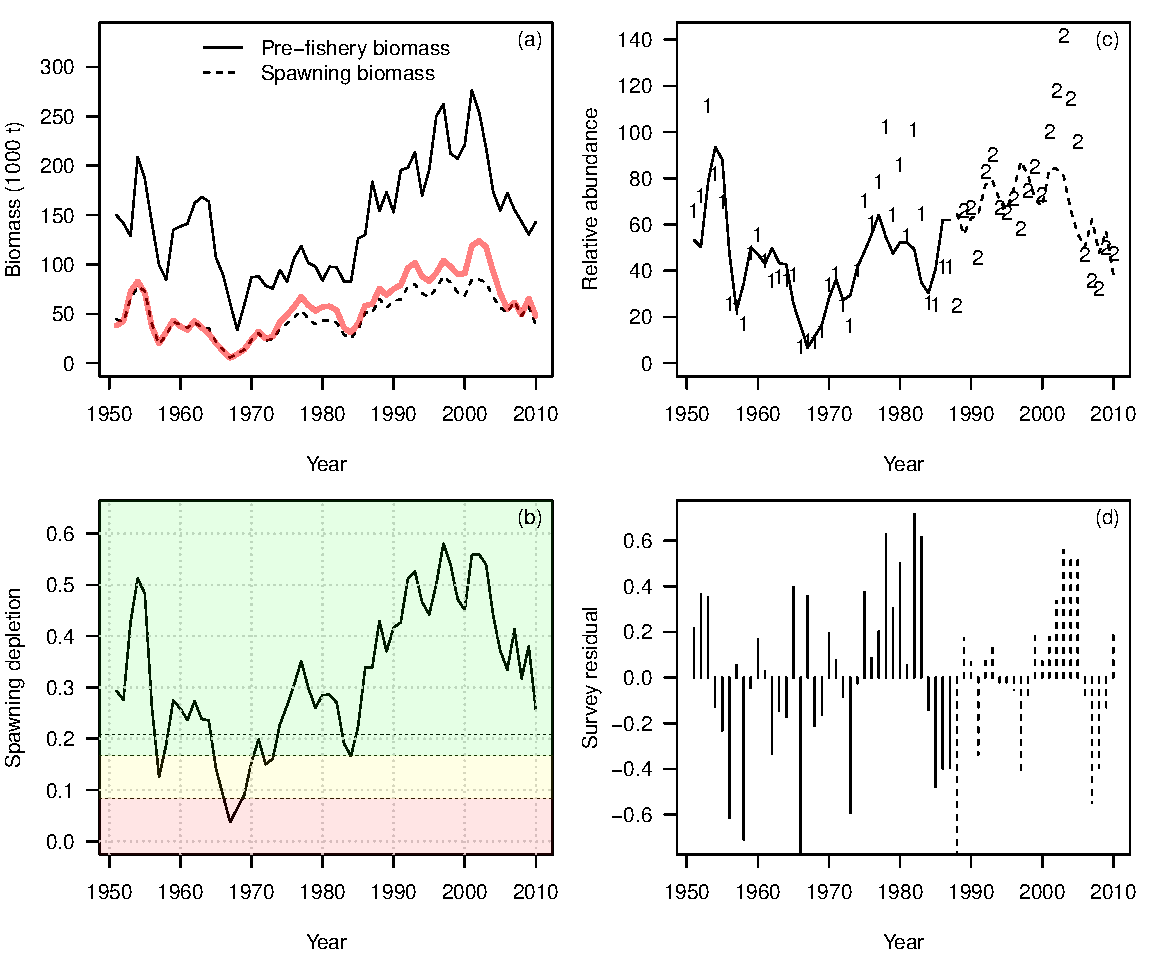
\includegraphics[width=\textwidth]{Figs/fig1_HCAM_ctrl.pdf}\\
	\caption{Maximum likelihood estimates of pre-fishery biomass and post fishery spawning biomass (a), spawning biomass depletion (b), observed (points) and predicted (lines) spawn survey data (c), and spawn survey residuals.  These results are based on trying to configure the \iscam\ model as similar as possible to the previous HCAM assessment; the red line in panel (a) is the MLE estimate of spawning biomass from HCAM.}\label{fig1_HCAM_ctrl}
\end{figure}


Estimates of the components of total mortality for the comparison with the HCAM model are shown in Figure \ref{fig2_HCAM_ctrl}.  The fishing mortality rates for each gear represent the average fishing mortality rate over all age-classes, and the natural mortality rate is assumed to be age-independent.  During the 1950s through to 1968, fishing mortality rates for Pacific herring in the Strait of Georgia were extremely high; this period was almost exclusively a purse-seine fishery where fish were taken for fishmeal.  After the fishery reopened in the early 1970s fishing mortality rates were greatly reduced and targeted the spawning component of the stock as the market was for herring roe. 

Estimates of natural mortality are based on a random walk process, initially starting at a value of 0.367 in 1951 and declining to a very low value of 0.068 in 1959, then increasing to a maximum of 1.02 in 1970 (Figure \ref{fig2_HCAM_ctrl}a).  Information to estimate natural mortality rates comes from the age-composition data, and assumptions about selectivity in the fishery.  In this comparison, the \iscam\ model assumes selectivity is invariant and much of the residual variation in the age-composition is explained by variation in $M$ and variation in age-2 recruits (see Figure \ref{fig3_HCAM_ctrl} for residual patterns and age-2 recruitment).  The HCAM model has a very similar trend in the estimates of natural mortality but the variability is much less than that of the \iscam\ assessment.  This is almost certainly due to the changes in selectivity for the gill net fishery associated with changes in mean body weight in the HCAM implementation.

There is good correspondence between the observed and predicted catch, however, the residual patterns does not appear to be iid for each of the fleets.  

 

\begin{figure}[!tbp]
	% Requires \usepackage{graphicx}
	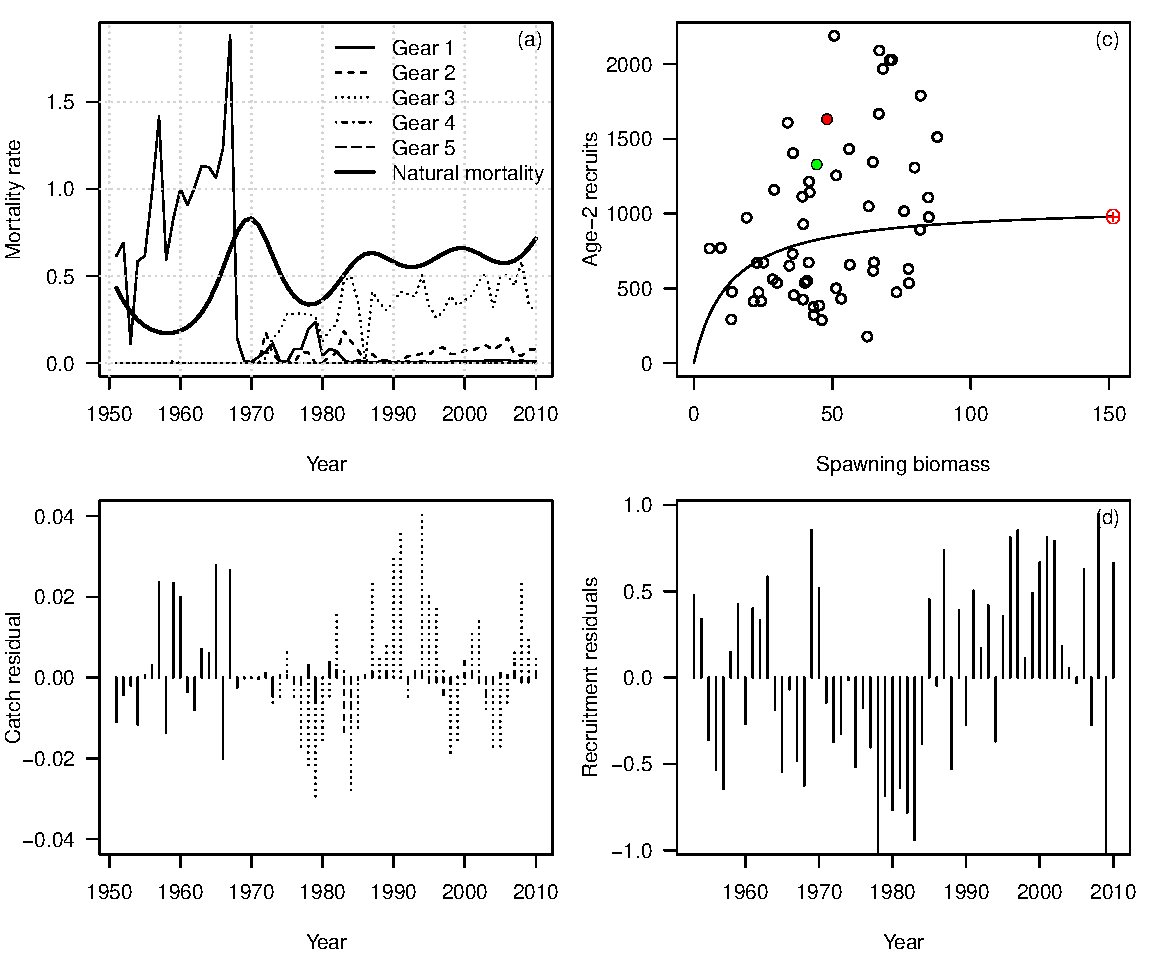
\includegraphics[width=\textwidth]{Figs/fig2_HCAM_ctrl.pdf}\\
	\caption{Components of total mortality rate (a), residuals between the observed and predicted catch (b), the spawning stock biomass versus age-2 recruits and stock recruitment relationship (estimates of unfished spawning biomass and unfished recruitment are denoted by the circle with the + symbol inside, c), and the residuals in the stock recruitment relationship (d). }\label{fig2_HCAM_ctrl}
\end{figure}

There was some lack of fit to the age-composition data for the purse seine fisheries and the best fits were actually obtained for the gill net fisheries. The conditional maximum likelihood estimates of the standard deviations of the age-composition data are 0.797, 0.672, and 0.326 for the winter purse seine, seine-roe, and gill net fisheries, respectively.  The smaller the standard deviation, the better correspondence between the observed and predicted age-composition data.

\begin{figure}[!tbp]
	% Requires \usepackage{graphicx}
	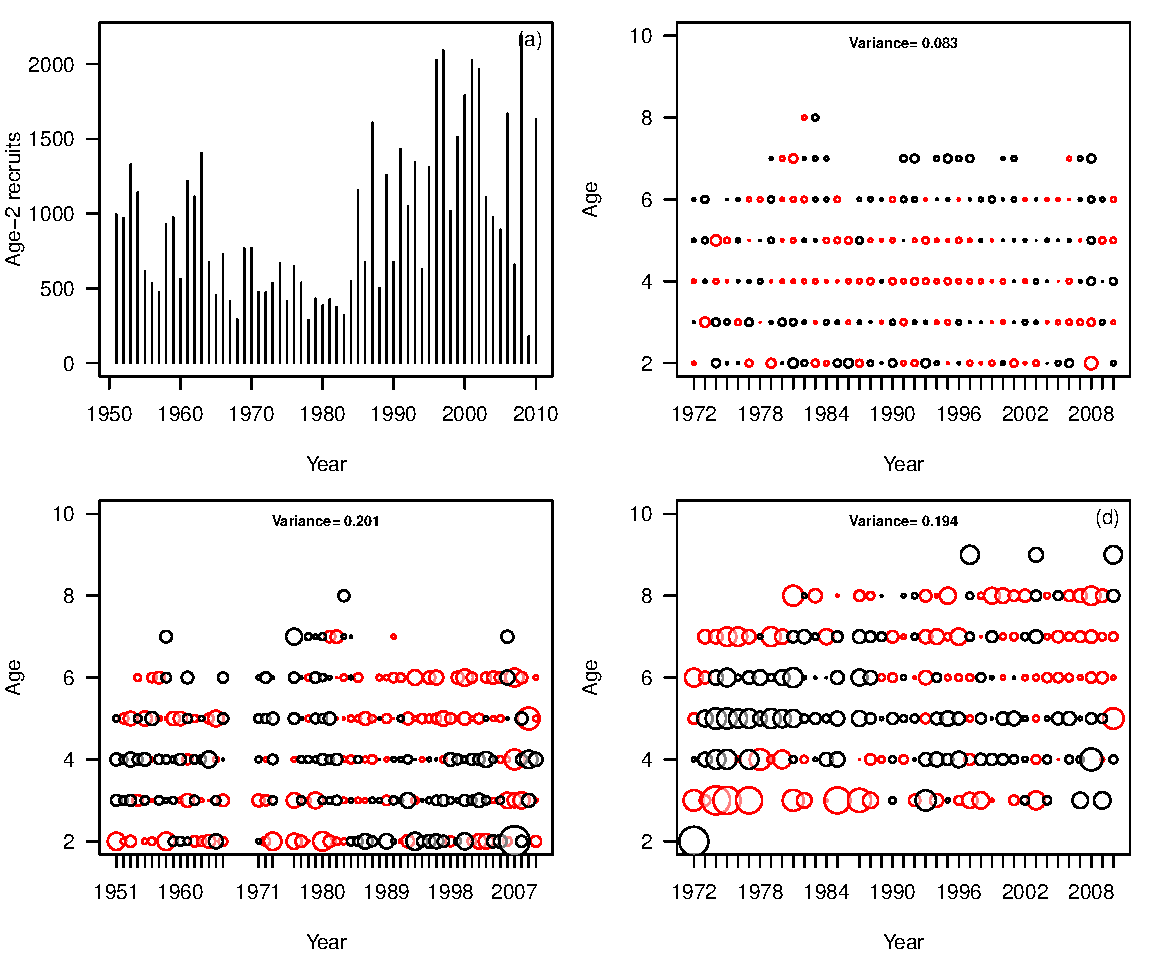
\includegraphics[width=\textwidth]{Figs/fig3_HCAM_ctrl.pdf}\\
	\caption{Estimates of age-2 recruits (a) and the residuals (observed-predicted, positive shown in black)  in the age-composition data for the winter purse seine fishery (lower left), seine-roe fishery (upper right) and gill net fishery (lower right). The area of each circle is proportional to the residual error, and zeros are not shown. Note that observed age-proportions less than 2\% were pooled into the adjacent (younger) age class and the conditional maximum likelihood estimates of the variance is displayed on the top of each panel.}\label{fig3_HCAM_ctrl}
\end{figure}

		\subsubsection{Strait of Georgia herring assessment}
		\subsubsection{Retrospective and prospective analyses}
	\subsection{Alternative assumptions about catchability, mortality \& selectivity}
		\subsubsection{Impacts of informative priors on $q$'s}
		\subsubsection{Implications of variable natural mortality rate $M_t$}
		\subsubsection{Implications of variable selectivity in directed fisheries}
	\subsection{Separating test fishery data from the purse seine roe fishery data}
	\subsection{Preliminary assessments for all other areas}
	
\begin{figure}[!tbp]
	% Requires \usepackage{graphicx}
	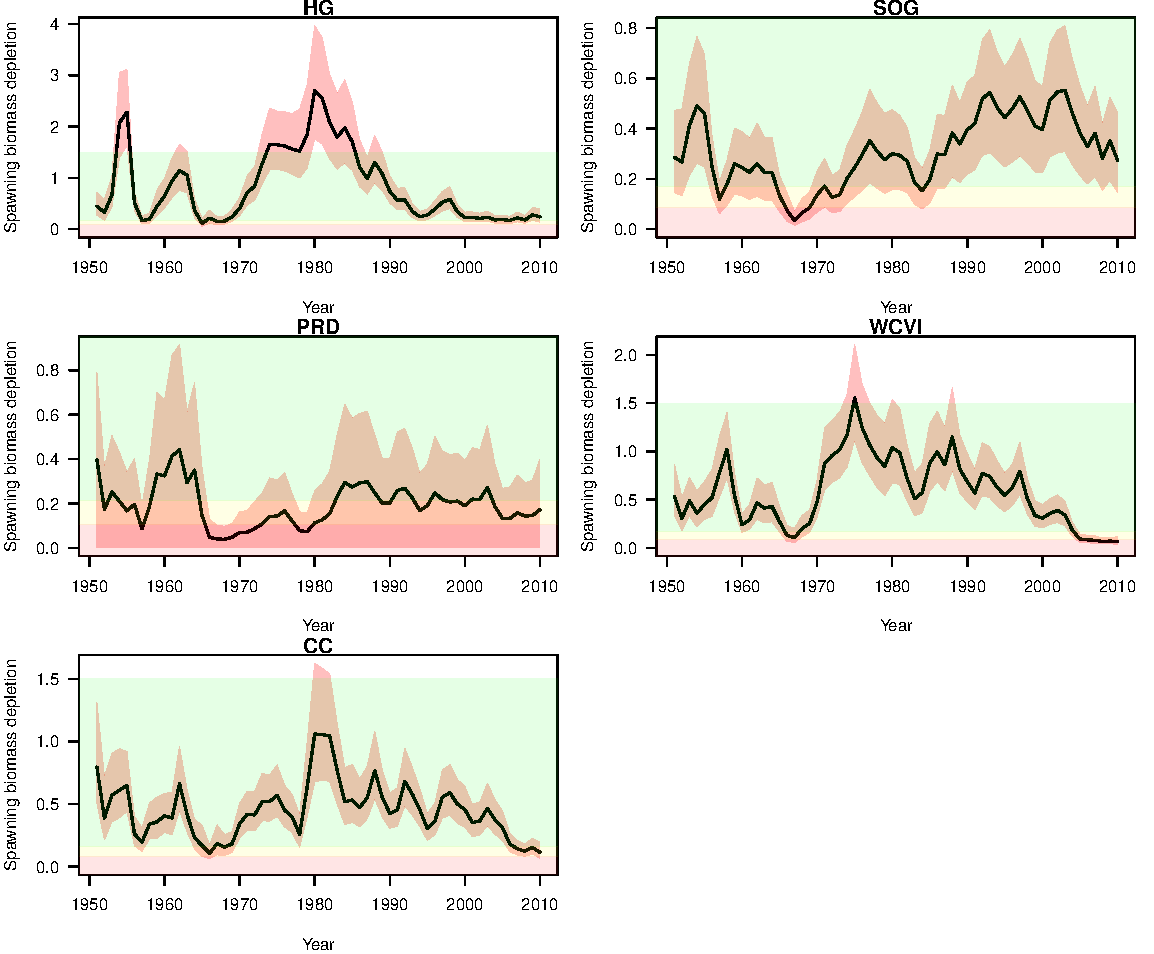
\includegraphics[width=\textwidth]{Figs/figSBmcmc.pdf}\\
	\caption{Cap.}\label{label}
\end{figure}
